\documentclass[../PianoDiProgetto.tex]{subfiles}
\begin{document}
	\section{Preventivo}
		\subsection{Analisi}
			\subsubsection{Prospetto orario}
			\begin{table}[H]
			\center
				\begin{tabular}{cccccccc}
				\noalign{\hrule height 1.5pt}
				\textbf{Nome} & \textbf{Res} & \textbf{Amm} & \textbf{An} & \textbf{Pt} & \textbf{Pr} & \textbf{Ve} & \textbf{Totale} \\ \hline
				Bonato Enrico & - & - & 5 & - & - & 5 & 10 \\ \hline
				Bonolo Marco  & - & - & 8 & - & - & - & 8 \\ \hline
				Pace Giulio  & - & 5 & 8 & - & - & 6 & 19 \\ \hline
				Pezzuto Francesco  & 2 & - & 9 & - & - & 8 & 19 \\ \hline
				Sanna Giovanni  & 2 & 4 & 7 & - & - & 5 & 18 \\ \hline
				Sovilla Matteo  & 8 & - & 7 & - & - & - & 15  \\ \hline
				\textbf{Ore Totali Ruolo} & \textbf{12} & \textbf{9} & \textbf{44} & \textbf{0} & \textbf{0} & \textbf{24} & \textbf{89} \\ \hline
				\noalign{\hrule height 1.5pt}
				\end{tabular}
			\caption{Prospetto orario Analisi.  \label{tab:table_label}}
			\end{table}
			\begin{figure}[H]
				\centering
				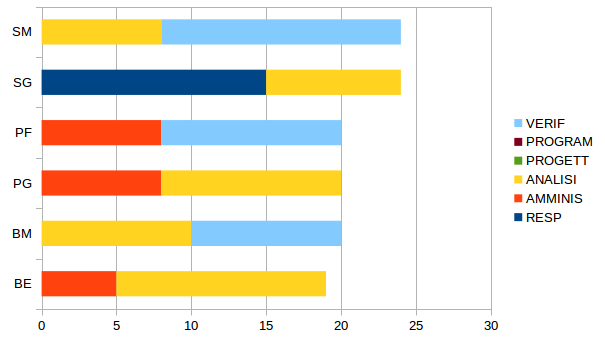
\includegraphics[scale=0.7]{Figures/OreComponenteAnalisi.png}
				\caption{Analisi: ore per componente.}\label{fig:1}
			\end{figure}
			\begin{figure}[H]
				\centering
				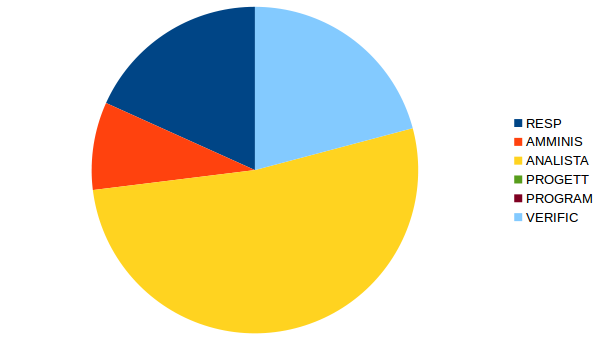
\includegraphics[scale=0.7]{Figures/OreRuoloAnalisi.png}
				\caption{Analisi: ore per ruolo.}\label{fig:2}
			\end{figure}
			
			\subsubsection{Prospetto economico}
			\begin{table}[H]
				\center
				\begin{tabular}{|c|c|c|}
					\noalign{\hrule height 1.5pt}
					\textbf{Ruolo} & \textbf{Ore} & \textbf{Costo(\euro)}     \\
					\hline
					Responsabile  & 12 & 360\\ 
					\hline
					Amministratore  & 9  & 180\\
					\hline
					Analista  & 44 & 1100\\
					\hline
					Progettista  & 0 & 0\\
					\hline
					Programmatore  & 0 & 0\\
					\hline
					Verificatore  & 24 & 360\\
					\hline
					\textbf{Totale}  & \textbf{89} & \textbf{2000}\\
					\noalign{\hrule height 1.5pt}
			\end{tabular}
			\caption{Prospetto economico Analisi.  \label{tab:table_label}}
		\end{table}
		
		\subsection{Analisi di dettaglio}
			\subsubsection{Prospetto orario} 
			\begin{table}[H]
			\center
				\begin{tabular}{cccccccc}
				\noalign{\hrule height 1.5pt}
				\textbf{Nome} & \textbf{Res} & \textbf{Amm} & \textbf{An} & \textbf{Pt} & \textbf{Pr} & \textbf{Ve} & \textbf{Totale} \\ \hline
				Bonato Enrico & - & - & - & - & - & 12 & 12 \\ \hline
				Bonolo Marco  & - & - & 10 & - & - & - & 10 \\ \hline
				Pace Giulio  & - & - & - & - & - & 12 & 12 \\ \hline
				Pezzuto Francesco  & - & - & 12 & - & - & - & 12 \\ \hline
				Sanna Giovanni  & - & - & 17 & - & - & - & 17 \\ \hline
				Sovilla Matteo  & 5 & 5 & - & - & - & 5 & 15 \\ \hline
				\textbf{Ore Totali Ruolo} & \textbf{5} & \textbf{5} & \textbf{39} & \textbf{0} & \textbf{0} & \textbf{29} & \textbf{78} \\ \hline
				\noalign{\hrule height 1.5pt}
				\end{tabular}
			\caption{Prospetto orario Analisi di dettaglio.  \label{tab:table_label}}
			\end{table}
			\begin{figure}[H]
				\centering
				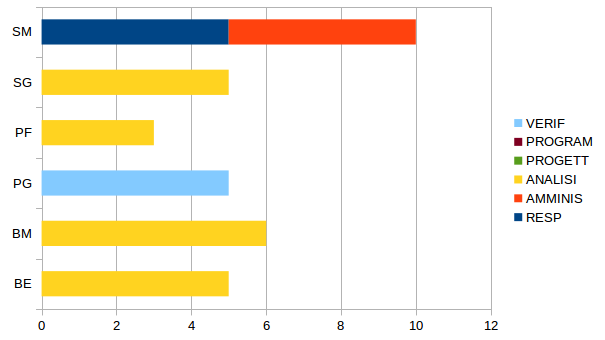
\includegraphics[scale=0.7]{Figures/OreComponenteAnalisiDett.png}
				\caption{Analisi di dettaglio: ore per componente.}\label{fig:4}
			\end{figure}
			\begin{figure}[H]
				\centering
				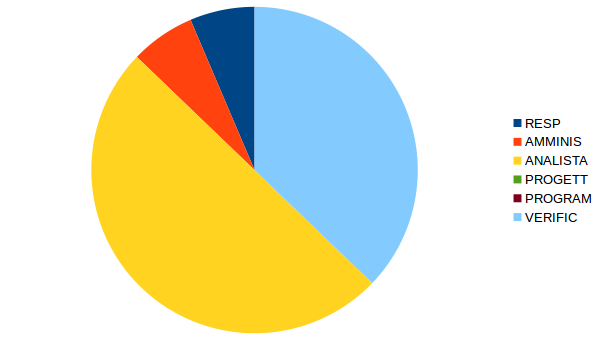
\includegraphics[scale=0.7]{Figures/OreRuoloAnalisiDett.png}
				\caption{Analisi di dettaglio: ore per ruolo.}\label{fig:5}
		\end{figure}
			
			\subsubsection{Prospetto economico}
			\begin{table}[H]
				\center
				\begin{tabular}{|c|c|c|}
					\noalign{\hrule height 1.5pt}
					\textbf{Ruolo} & \textbf{Ore} & \textbf{Costo(\euro)}     \\
					\hline
					Responsabile  & 5 & 150 \\
					\hline
					Amministratore  & 5  & 100 \\
					\hline
					Analista  & 39  & 975\\
					\hline
					Progettista  & 0 & 0\\
					\hline
					Programmatore  & 0 & 0\\
					\hline
					Verificatore  & 29 & 435\\
					\hline
					\textbf{Totale}  & \textbf{78} & \textbf{1660}\\
					\noalign{\hrule height 1.5pt}
			\end{tabular}
			\caption{Prospetto economico Analisi di dettaglio.  \label{tab:table_label}}
		\end{table}
		
		
		\subsection{Progettazione architetturale}
			\subsubsection{Prospetto orario}
			\begin{table}[H]
			\center
				\begin{tabular}{cccccccc}
				\noalign{\hrule height 1.5pt}
				\textbf{Nome} & \textbf{Res} & \textbf{Amm} & \textbf{An} & \textbf{Pt} & \textbf{Pr} & \textbf{Ve} & \textbf{Totale} \\ \hline
				Bonato Enrico & 6 & - & 14 & 14 & - & - & 34 \\ \hline
				Bonolo Marco  & - & 10 & - & - & - & 26 & 36 \\ \hline
				Pace Giulio  & 6 & - & 15 & 12 & - & - & 33 \\ \hline
				Pezzuto Francesco  & - & - & 15 & 14 & - & - & 29 \\ \hline
				Sanna Giovanni  & - & 13 & - & - & - & 18 & 31 \\ \hline
				Sovilla Matteo  & - & - & 21 & 16 & - & - & 37 \\ \hline
				\textbf{Ore Totali Ruolo} & \textbf{12} & \textbf{23} & \textbf{65} & \textbf{56} &  \textbf{0}& \textbf{44} & \textbf{200} \\ \hline
				\noalign{\hrule height 1.5pt}
				\end{tabular}
			\caption{Prospetto orario Progettazione architetturale.  \label{tab:table_label}}
			\end{table}
			\begin{figure}[H]
				\centering
				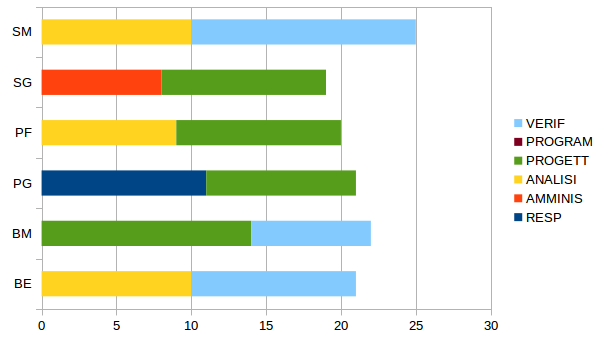
\includegraphics[scale=0.7]{Figures/OreComponenteProgArch.png}
				\caption{Progettazione architetturale: ore per componente.}\label{fig:7}
			\end{figure}
			\begin{figure}[H]
				\centering
				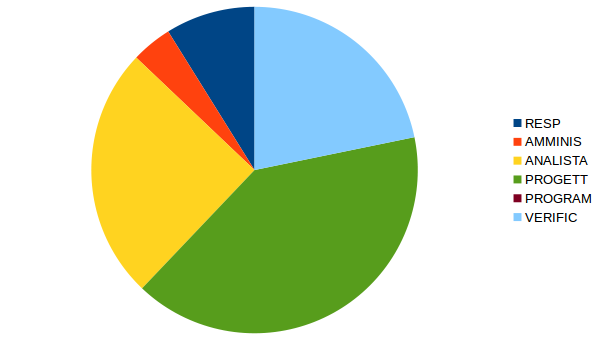
\includegraphics[scale=0.7]{Figures/OreRuoloProgArch.png}
				\caption{Progettazione architetturale: ore per ruolo.}\label{fig:8}
			\end{figure}
			
			\subsubsection{Prospetto economico}
			\begin{table}[H]
				\center
				\begin{tabular}{|c|c|c|}
					\noalign{\hrule height 1.5pt}
					\textbf{Ruolo} & \textbf{Ore} & \textbf{Costo(\euro)}     \\
					\hline
					Responsabile  & 12 & 360 \\
					\hline
					Amministratore  &  23 & 460 \\
					\hline
					Analista  & 65 & 1625 \\
					\hline
					Progettista  & 56 & 1232 \\
					\hline
					Programmatore  & 0 & 0 \\
					\hline 
					Verificatore  & 44 & 660 \\
					\hline
					\textbf{Totale}  & \textbf{200} & \textbf{4337}\\
					\noalign{\hrule height 1.5pt}
			\end{tabular}
			\caption{Prospetto economico Progettazione architetturale.  \label{tab:table_label}}
		\end{table}
		
		
		\subsection{Progettazione di dettaglio e Codifica}
			\subsubsection{Prospetto orario}
			\begin{table}[H]
			\center
				\begin{tabular}{cccccccc}
				\noalign{\hrule height 1.5pt}
				\textbf{Nome} & \textbf{Res} & \textbf{Amm} & \textbf{An} & \textbf{Pt} & \textbf{Pr} & \textbf{Ve} & \textbf{Totale} \\ \hline
				Bonato Enrico & - & 12 & - & 21 & 15 & - & 48 \\ \hline
				Bonolo Marco  & 8 & - & 10 & - & 15 & 26 & 59 \\ \hline
				Pace Giulio  & - & - & - & 17 & 17 & 23 & 57 \\ \hline
				Pezzuto Francesco  & 4 & 5 & - & 16 & 14 & 20 & 59 \\ \hline
				Sanna Giovanni  & - & - & 8 & 19 & 14 & 18 & 59 \\ \hline
				Sovilla Matteo  & - & - & 6 & 26 & 14 & - & 46 \\ \hline
				\textbf{Ore Totali Ruolo} & \textbf{12} & \textbf{17} & \textbf{24} & \textbf{99} & \textbf{89} & \textbf{87} & \textbf{328} \\ \hline
				\noalign{\hrule height 1.5pt}
				\end{tabular}
			\caption{Prospetto orario Progettazione di dettaglio e Codifica.  \label{tab:table_label}}
			\end{table}
			\begin{figure}[H]
				\centering
				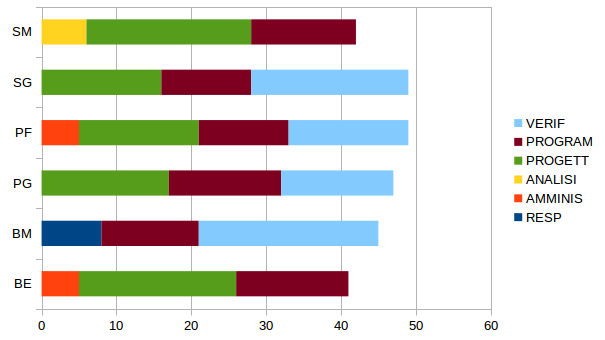
\includegraphics[scale=0.7]{Figures/OreComponenteProgDettCodifica.png}
				\caption{Progettazione di dettaglio e codifica: ore per componente.}\label{fig:10}
			\end{figure}
			\begin{figure}[H]
				\centering
				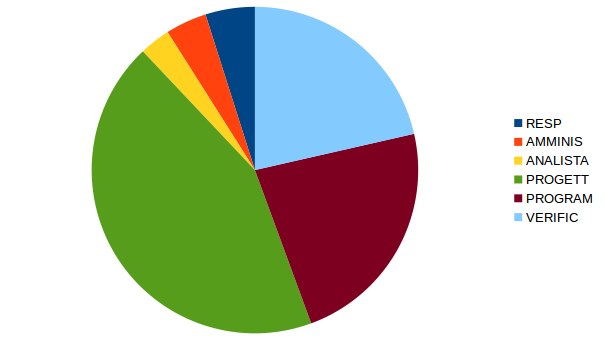
\includegraphics[scale=0.7]{Figures/OreRuoloProgDettCodifica.png}
				\caption{Progettazione di dettaglio e codifica: ore per ruolo.}\label{fig:11}
			\end{figure}
			
			\subsubsection{Prospetto economico}
			\begin{table}[H]
				\center
				\begin{tabular}{|c|c|c|}
					\noalign{\hrule height 1.5pt}
					\textbf{Ruolo} & \textbf{Ore} & \textbf{Costo(\euro)}     \\
					\hline
					Responsabile  & 12 & 360\\
					\hline
					Amministratore  & 17  & 340 \\
					\hline
					Analista  & 24  & 600 \\
					\hline
					Progettista  & 99 & 2178 \\
					\hline
					Programmatore  & 89 & 1335 \\
					\hline
					Verificatore  & 87 & 1305 \\
					\hline
					\textbf{Totale}  & \textbf{328} & \textbf{6118}\\
					\noalign{\hrule height 1.5pt}
			\end{tabular}
			\caption{Prospetto economico Progettazione di dettaglio e Codifica.  \label{tab:table_label}}
		\end{table}
		
		\subsection{Validazione}
			\subsubsection{Prospetto orario}
			\begin{table}[H]
			\center
				\begin{tabular}{cccccccc}
				\noalign{\hrule height 1.5pt}
				\textbf{Nome} & \textbf{Res} & \textbf{Amm} & \textbf{An} & \textbf{Pt} & \textbf{Pr} & \textbf{Ve} & \textbf{Totale} \\ \hline
				Bonato Enrico & - & - & - & 8 & 0 & 15 & 23 \\ \hline
				Bonolo Marco  & - & - & - & 4 & 6 & - & 10 \\ \hline
				Pace Giulio  & - & - & - & - & 6 & 9 & 15 \\ \hline
				Pezzuto Francesco  & - & 8 & - & - & - & 9 & 17 \\ \hline
				Sanna Giovanni  & 8 & - & - & - & 7 & - & 15 \\ \hline
				Sovilla Matteo  & - & - & - & - & - & 22 & 22 \\ \hline
				\textbf{Ore Totali Ruolo} & \textbf{8} & \textbf{8} & \textbf{0} & \textbf{12} & \textbf{19} & \textbf{55} & \textbf{102} \\ \hline
				\noalign{\hrule height 1.5pt}
				\end{tabular}
			\caption{Prospetto orario Validazione.  \label{tab:table_label}}
			\end{table}
			\begin{figure}[H]
				\centering
				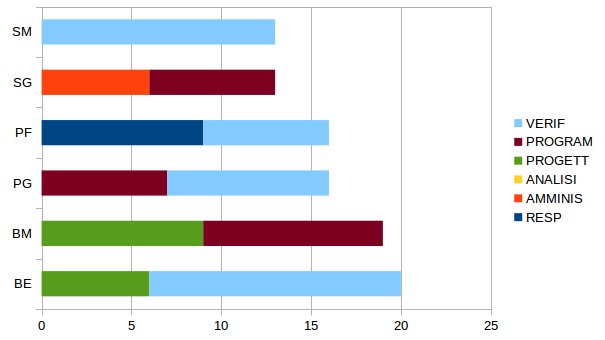
\includegraphics[scale=0.7]{Figures/OreComponenteValidazione.png}
				\caption{Validazione: ore per componente.}\label{fig:13}
			\end{figure}
			\begin{figure}[H]
				\centering
				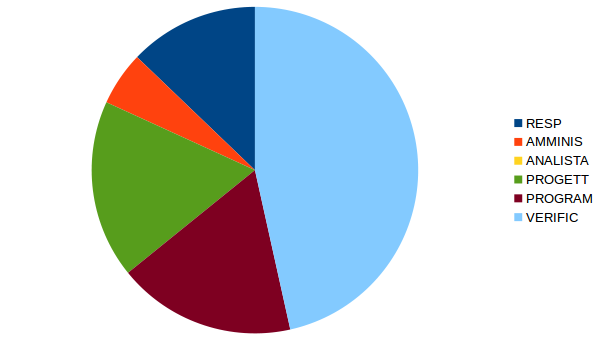
\includegraphics[scale=0.7]{Figures/OreRuoloValidazione.png}
				\caption{Validazione: ore per ruolo.}\label{fig:14}
			\end{figure}
			
			\subsubsection{Prospetto economico}
			\begin{table}[H]
				\center
				\begin{tabular}{|c|c|c|}
					\noalign{\hrule height 1.5pt}
					\textbf{Ruolo} & \textbf{Ore} & \textbf{Costo(\euro)}     \\
					\hline
					Responsabile  & 8 & 270 \\
					\hline
					Amministratore  & 8  & 160 \\
					\hline
					Analista  & 0  & 0 \\
					\hline
					Progettista  & 12 & 264 \\
					\hline
					Programmatore  & 19  & 285\\ 
					\hline
					Verificatore  & 55 & 825 \\
					\hline
					\textbf{Totale}  & \textbf{102} & \textbf{1804}\\
					\noalign{\hrule height 1.5pt}
			\end{tabular}
			\caption{Prospetto economico Validazione.  \label{tab:table_label}}
		\end{table}
		
	\subsection{Riepilogo}
		\subsubsection{Prospetto orario}
		\begin{table}[H]
			\center
				\begin{tabular}{cccccccc}
				\noalign{\hrule height 1.5pt}
				\textbf{Nome} & \textbf{Res} & \textbf{Amm} & \textbf{An} & \textbf{Pt} & \textbf{Pr} & \textbf{Ve} & \textbf{Totale} \\ \hline
				Bonato Enrico & 6 & 12 & 14 & 43 & 15 & 15 & 105 \\ \hline
				Bonolo Marco  & 8 & 10 & 10 & 4 & 21 & 52 & 105 \\ \hline
				Pace Giulio  & 6 & 0 & 15 & 29 & 23 & 32 & 105  \\ \hline
				Pezzuto Francesco  & 4 & 13 & 15 & 29 & 23 & 32 & 105 \\ \hline
				Sanna Giovanni  & 8 & 13 & 8 & 19 & 21 & 36 & 105 \\ \hline
				Sovilla Matteo  & 0 & 0 & 27 & 42 & 14 & 22 & 105 \\ \hline
				\textbf{Ore Totali Ruolo} & \textbf{32} & \textbf{48} & \textbf{89} & \textbf{167} & \textbf{108} & \textbf{186} & \textbf{630} \\ \hline
				\noalign{\hrule height 1.5pt}
				\end{tabular}
			\caption{Riepilogo prospetto orario.  \label{tab:table_label}}
			\end{table}
		\begin{figure}[H]
			\centering
			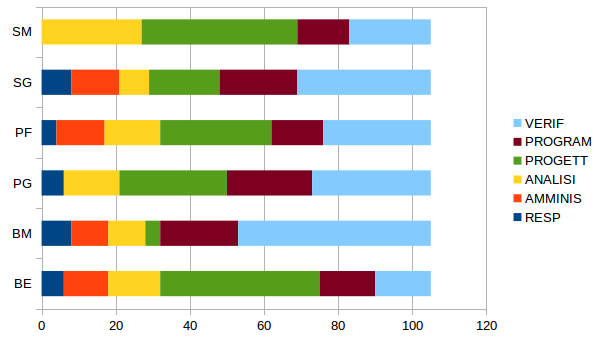
\includegraphics[scale=0.7]{Figures/OreComponenteRiepilogoRend.png}
			\caption{Riepilogo: ore rendicontate per componente.}\label{fig:15}
		\end{figure}
		\begin{figure}[H]
			\centering
			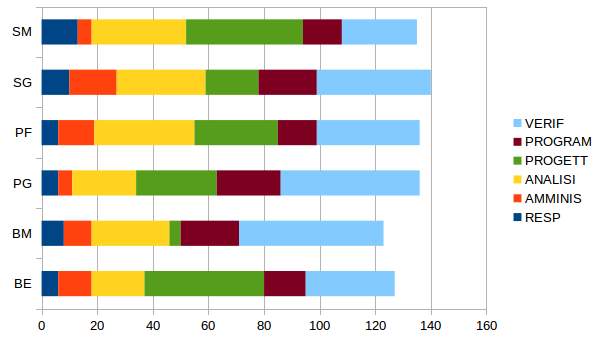
\includegraphics[scale=0.7]{Figures/OreComponenteRiepilogoTot.png}
			\caption{Riepilogo: ore totali per componente.}\label{fig:15}
		\end{figure}
		\begin{figure}[H]
			\centering
			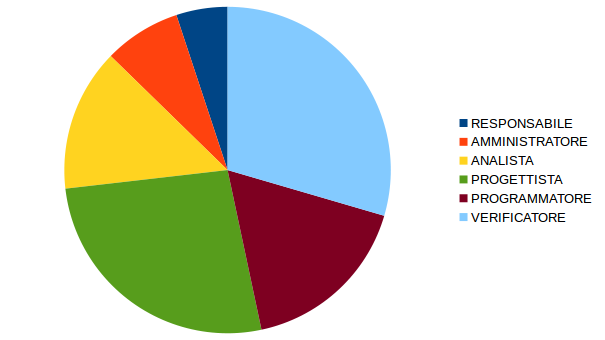
\includegraphics[scale=0.7]{Figures/OreRuoloRiepilogoRend.png}
			\caption{Riepilogo: ore rendicontate per ruolo.}\label{fig:5}
		\end{figure}
		\begin{figure}[H]
			\centering
			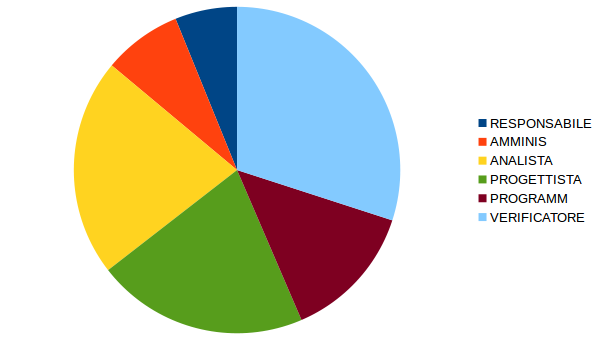
\includegraphics[scale=0.7]{Figures/OreRuoloRiepilogoTot.png}
			\caption{Riepilogo: ore totali per ruolo.}\label{fig:5}
		\end{figure}
			
		\subsubsection{Prospetto economico}
			\begin{table}[H]
				\center
				\begin{tabular}{|c|c|c|}
					\noalign{\hrule height 1.5pt}
					\textbf{Ruolo} & \textbf{Ore} & \textbf{Costo(\euro)}     \\
					\hline
					Responsabile  & 32 & 960 \\ 
					\hline
					Amministratore  & 48  & 960 \\
					\hline
					Analista  & 89  & 2225 \\ 
					\hline
					Progettista  & 167 & 3674\\
					\hline
					Programmatore  & 108  & 1620\\
					\hline
					Verificatore  & 186 & 2790\\
					\hline
					\textbf{Totale}  & \textbf{630} & \textbf{12229}\\
					\noalign{\hrule height 1.5pt}
			\end{tabular}
			\caption{Riepilogo prospetto economico.  \label{tab:table_label}}
		\end{table}
		
\end{document}
